\documentclass{homework}
\usepackage{homework}
\usepackage{hanhua}
\title{report}
\subtitle{week 5}
\begin{document}

\maketitle
\section{myAtio.h}
\subsection{函数说明}
将含有数字的字符串转化为对应整数。
\paragraph{输入}
一个字符串。
\paragraph{输出}
一个整形:字符串转换的结果,或0(字符串不合法)。
\paragraph{实现方法}
\begin{itemize}
    \item 首先将检查指针移到第一个非空白字符(非空格、制表符、换行符)上,
    \item 若检测到‘+’, ‘-’, 或者数字则标记为开始数字,并记录符号,否则直接返回零(不合法字符)。
    \item 开始数字后,只能检测到数字字符,并且每次检测后采用左移后相加的方法更新数字;若检测到非数字字符直接跳出检测环节。
    \item 最后乘上符号,得到转换后的整数。
\end{itemize}
\subsection{复杂度}
\paragraph{时间复杂度}
$\mathcal{O}(n)$
\paragraph{空间复杂度}
$\mathcal{O}(1)$
\subsection{边界情况}
\begin{itemize}
    \item 若传入空指针/空字符串,直接返回0。
    \item 判断数字越界:其实可以通过先使用长整形来更新数字,每次更新后用大于号、小于号判断是否越界,越界则用指定的INT\_MAX、INT\_MIN替换,最后转为整形返回。但考虑到需要数字不超过整形的范围有可能是为了兼容不同字长的计算机,于是采用如下方法:

          在左移(十进制左移)前先判断更新前的数字在更新后是否越界(分别比较前面和最后一位),若越界则返回相应符号的替代值,否则可以继续更新。
    \item 由例子可以看出,对于有前导零的数字仍处理为十进制而非八进制,对于十六进制、科学计数法则忽略了‘x’, ‘e’或小数点及其后的字符。故在本程序中无需做更多处理。
\end{itemize}
\subsection{程序运行结果}
\begin{figure}[H]
    \centering
    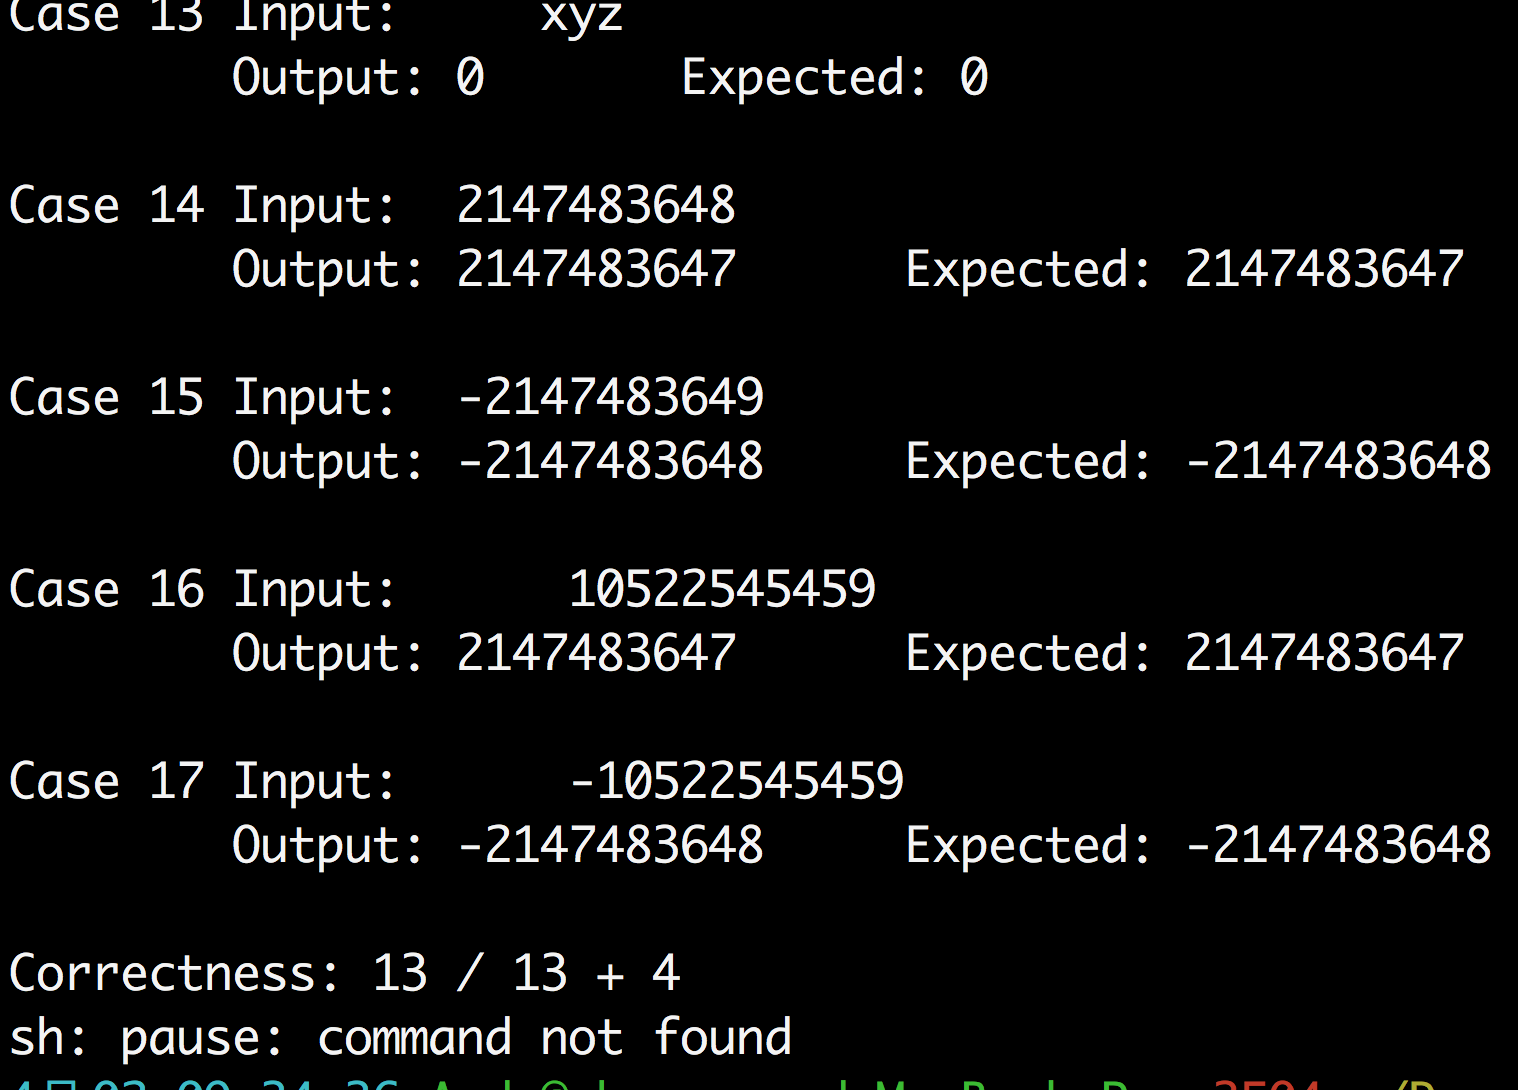
\includegraphics[width=7cm]{atoi.png}
\end{figure}
\section{evalRPN.h}
\subsection{函数说明}
将一系列含有数字或运算符的字符串按照逆波兰表示法计算表达式并返回结果。
\paragraph{输入}
一个指向含有一系列字符串指针的指针。
\paragraph{输出}
一个整数:将输入的这系列字符串转换为相对应的数字或符号,并按逆波兰表示法计算该表达式的结果。
\paragraph{实现方法}
实现方法在题目中已经给出。用栈实现:若检测到数字则压栈,若检测到符号则将栈顶两元素弹出,进行对应运算后再压入。合法的表达式最终会得到仅有一元的栈,即要返回的值。

对数字串的转换则由myAtoi.h改进得到。
\subsection{复杂度}
\paragraph{时间复杂度}
$\mathcal{O}(n)$
\paragraph{空间复杂度}
$\mathcal{O}(n)$
\subsection{边界情况}
\begin{itemize}
    \item 若输入为空指针,返回0。
    \item 若字符串系列里出现空字符串,则视为不合法直接返回0,而非忽略之。
    \item 根据题意,运算符只能为“+”, “-”, “*”, “/”四种,“.*”(点乘)“  *  ”(有空格)“*”(全角)“×”(乘法符号)这些形式都不被许可,会被当作高容忍量的数字串进行转换(并失败然后返回0)。
    \item 在转换数字串时若转换失败则直接返回0。
    \item 若数字越界仍采取和myAtoi.h中同样的处理方式,但由于在本题中会发生越界的数再次运算的情况,所以其实这种做法仅在只有最后一步运算发生0和越界数运算的情况才有意义,否则将返回不准确的结果。
    \item 栈溢出:压栈时超过栈最大容量MAXSIZE,报错栈溢出并返回0。
    \item 若在栈中元素不足两个时检测到运算符号,则发生invalid operator错误并返回0。
    \item 成功处理完整个系列后,若栈中有多个元素,则发生extra number错误并返回0。
    \item 作为一个可能被反复调用的转换函数,本程序抑制了所有报错信息,故正确的运算结果0和错误0并不被区分。
\end{itemize}
\subsection{程序运行结果}
\begin{figure}[H]
    \centering
    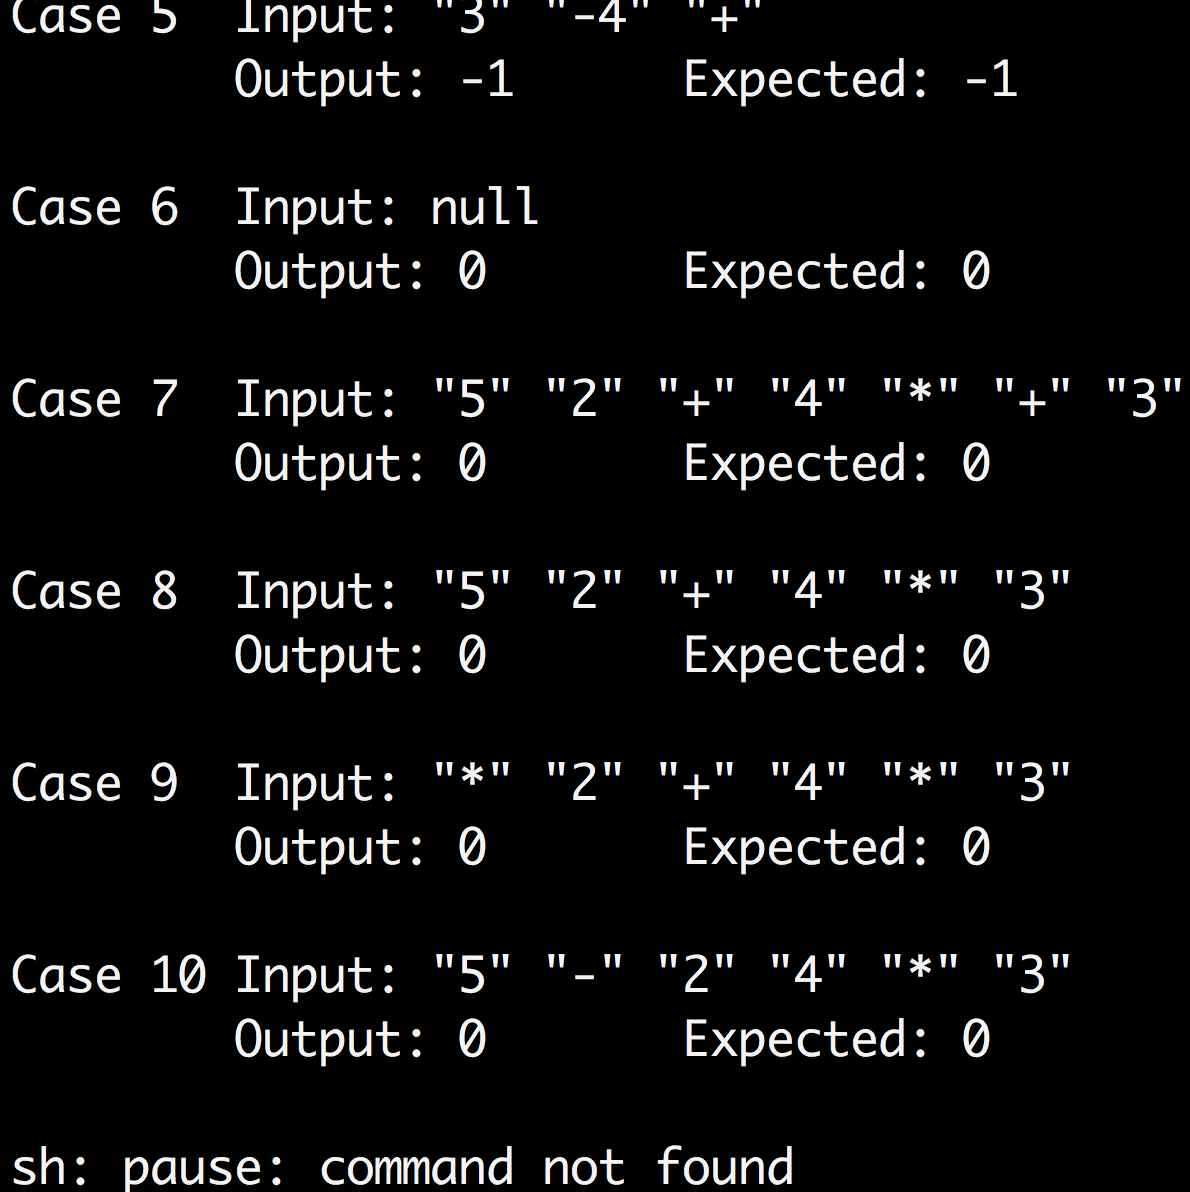
\includegraphics[width=7cm]{eval.png}
\end{figure}
\end{document}
